\documentclass[10pt,twocolumn,letterpaper]{article}

% --- Typography & Geometry ---
\usepackage[utf8]{inputenc}
\usepackage{microtype}
\usepackage[margin=0.75in,top=0.85in,bottom=0.85in]{geometry}

% --- Math & Symbols ---
\usepackage{amsmath,amssymb,amsfonts,amsthm}
\usepackage{bm}

% --- Tables & Arrays ---
\usepackage{booktabs}
\usepackage{tabularx}
\usepackage{array}

% --- Graphics & Floats ---
\usepackage{graphicx}
\usepackage{float}
\usepackage{subcaption}

% --- Code Listings ---
\usepackage{xcolor}
\usepackage{listings}

\definecolor{codebg}{HTML}{F8F9FA}
\definecolor{codeframe}{HTML}{D0D7DE}
\definecolor{keywordcolor}{HTML}{0550AE}
\definecolor{stringcolor}{HTML}{0A3069}
\definecolor{commentcolor}{HTML}{57606A}

\lstset{
    backgroundcolor=\color{codebg},
    basicstyle=\ttfamily\scriptsize\color{black},
    keywordstyle=\color{keywordcolor}\bfseries,
    stringstyle=\color{stringcolor},
    commentstyle=\color{commentcolor}\itshape,
    frame=single,
    rulecolor=\color{codeframe},
    breaklines=true,
    breakatwhitespace=true,
    extendedchars=true,
    xleftmargin=6pt,
    xrightmargin=6pt,
    aboveskip=8pt,
    belowskip=8pt
}

% --- Hyperlinks ---
\usepackage{hyperref}
\hypersetup{
    colorlinks=true,
    linkcolor=blue!70!black,
    citecolor=blue!70!black,
    urlcolor=blue!70!black
}

% --- Input Title & Authors ---
% Metadata for padre_attention
\title{\textbf{PADRe: Polynomial Attention with Dropout Regularization for Multi-Architecture Transformers}}

\author{
  \textbf{Taha Majs}\thanks{Corresponding author: tahamajs@uni.edu} \quad \textbf{Research Team} \\
  Department of Computer Science \\
  Advanced Machine Learning \& Efficiency Laboratory
}

\date{\today}


\begin{document}

\maketitle

% --- Abstract & Keywords Block ---
\begin{abstract}
We introduce \textbf{PADRe} (\textbf{P}olynomial \textbf{A}ttention with \textbf{D}ropout \textbf{R}egularization), 
a multi-architecture attention module that replaces the softmax normalization 
of standard attention with a \textbf{polynomial kernel}:

\[
\text{attn}(q_i, k_j) = \frac{(1 + s_{ij}/\text{order})^\text{order}}{\sum_{j'} (1 + s_{ij'}/\text{order})^\text{order}}
\]

where $s_{ij}$ is the scaled, centered dot-product score. This polynomial 
kernel is a \textbf{Taylor approximation} of $\exp(s)$ and, unlike softmax, is 
\textbf{kernelizable} -- it can be expressed as $\phi(q) \cdot \phi(k)$ where $\phi$ 
is a finite-dimensional feature map. This property has the potential to enable 
$\mathcal{O}(N)$ attention.

\textbf{However, the current implementation is not kernelized.} The attention 
weights are materialized as an $[N \times N]$ matrix, so the runtime is 
$\mathcal{O}(N^2 d_h)$ -- identical to standard softmax attention. The 
polynomial kernel does not, by itself, provide speedup without the 
corresponding kernelization step.

\textbf{What PADRe does provide:}

\begin{enumerate}
\item \textbf{Numerical stability via max-centering} of scores over valid positions,
  preventing overflow in the polynomial expansion.
\item \textbf{Dropout regularization} on the polynomial attention weights.
\item \textbf{Multi-architecture support} across DistilBERT, RoBERTa, GPT-2, and Qwen.
\item \textbf{Frobenius-norm weight-copy validation} with output-equivalence check.
\item \textbf{Nested encoder bypass} for RoBERTa-style architectures.

\end{enumerate}
On SST-2, PADRe achieves \textbf{{{D\_ACC}}\%} on DistilBERT (baseline {{BASE\_D}}\%, 
$\Delta$ = {{D\_DELTA}}), \textbf{{{R\_ACC}}\%} on RoBERTa (baseline {{BASE\_R}}\%, 
$\Delta$ = {{R\_DELTA}}), and \textbf{{{G\_ACC}}\%} on GPT-2 (baseline {{BASE\_G}}\%, 
$\Delta$ = {{G\_DELTA}}), using {{RECOVERY\_STEPS}} LoRA recovery steps. We 
position PADRe as a \textbf{research module} for exploring polynomial attention 
in pretrained transformers, with the kernelization step explicitly left to 
future work.

\textbf{Keywords:} polynomial attention, kernelized attention, Taylor approximation, 
softmax replacement, multi-architecture



\vspace{0.5em}
\noindent\textbf{Keywords:} polynomial attention, kernelized attention, Taylor approximation,
\end{abstract}

\vspace{1em}

% --- Paper Body ---
\section{01 Intro}

Formal architectural specifications for \texttt{padre_attention}.

\section{Related Work}

\subsection{Kernelized Attention}

\textbf{Performer} (Choromanski et al., 2021) uses **positive orthogonal random 
features (PORF)** to approximate the softmax kernel. 

\textbf{Linear Transformer} (Katharopoulos et al., 2020) uses $\phi(x) = \text{elu}(x) + 1$.

\textbf{Random Feature Attention} (Peng et al., 2021) uses Gaussian RFF.

\textbf{Our distinction.} PADRe uses a \textbf{deterministic polynomial kernel} -- no 
randomness. This is more stable but restricts the kernel family.

\subsection{Polynomial Attention}

\textbf{Poly-NL} (Choromanski et al., 2021) uses polynomial features 
$\phi(x) = (1, x, x^2, \dots)$ for kernelized attention. 

\textbf{Kacham et al. (2024)} analyze polynomial attention approximation bounds.

\textbf{Our distinction.} PADRe uses a specific degree-$d$ kernel with max-centering 
for stability, applied to pretrained models with LoRA recovery.

\subsection{Softmax Alternatives}

\textbf{Sigmoid Attention} (Ramapuram et al., 2024) uses element-wise sigmoid 
in place of softmax. \textbf{Softpick} (Zuhri et al., 2025) uses a rectified 
exponential. \textbf{Softmax Linear Units} (Softermax, 2023) uses a bounded base.

\textbf{Our distinction.} PADRe specifically targets the polynomial approximation 
family with an explicit kernelization path.

\subsection{Pretrained Model Adaptation}

\textbf{LoRA} (Hu et al., 2021), \textbf{AdaLoRA} (Zhang et al., 2023), \textbf{DoRA} 
(Liu et al., 2024) provide parameter-efficient fine-tuning. Our work uses 
LoRA for post-substitution recovery.

\subsection{Position of Our Work}

\begin{table}[H]
\centering
\small
\begin{tabular}{llll}
\toprule
\textbf{Method} & \textbf{Kernel Family} & \textbf{Kernelized} & \textbf{Pretrained} \\
\midrule
Softmax & exponential &  & -- \\
Performer & RFF &  &  \\
Linear Transformer & elu+1 &  &  \\
Poly-NL & polynomial &  &  \\
\textbf{PADRe} & \textbf{polynomial} & \textbf{Partial} & \textbf{ } \\
\bottomrule
\end{tabular}
\end{table}

\textbf{Key distinction.} PADRe is the first to apply polynomial-kernel attention 
to pretrained transformers with multi-architecture weight transfer and 
LoRA recovery.



\subsection{Comparison Table}

\begin{table}[H]
\centering
\small
\begin{tabular}{llll}
\toprule
\textbf{Method} & \textbf{Complexity} & \textbf{Stable?} & \textbf{Pretrained} \\
\midrule
Softmax & $\mathcal{O}(N^2 d_h)$ &  & -- \\
Performer & $\mathcal{O}(N F d_h)$ & Varies &  \\
Poly-NL & $\mathcal{O}(N F d_h)$ &  &  \\
\textbf{PADRe (unser kernelized)} & $\mathcal{O}(N^2 d_h)$ &  & \textbf{ } \\
PADRe (kernelized, future) & $\mathcal{O}(N F d_h)$ &  &  \\
\bottomrule
\end{tabular}
\end{table}


\section{03 Background}

Formal architectural specifications for \texttt{padre_attention}.

\section{04 Method}

Formal architectural specifications for \texttt{padre_attention}.

\section{05 Architecture}

Formal architectural specifications for \texttt{padre_attention}.


\begin{figure}[H]
\centering
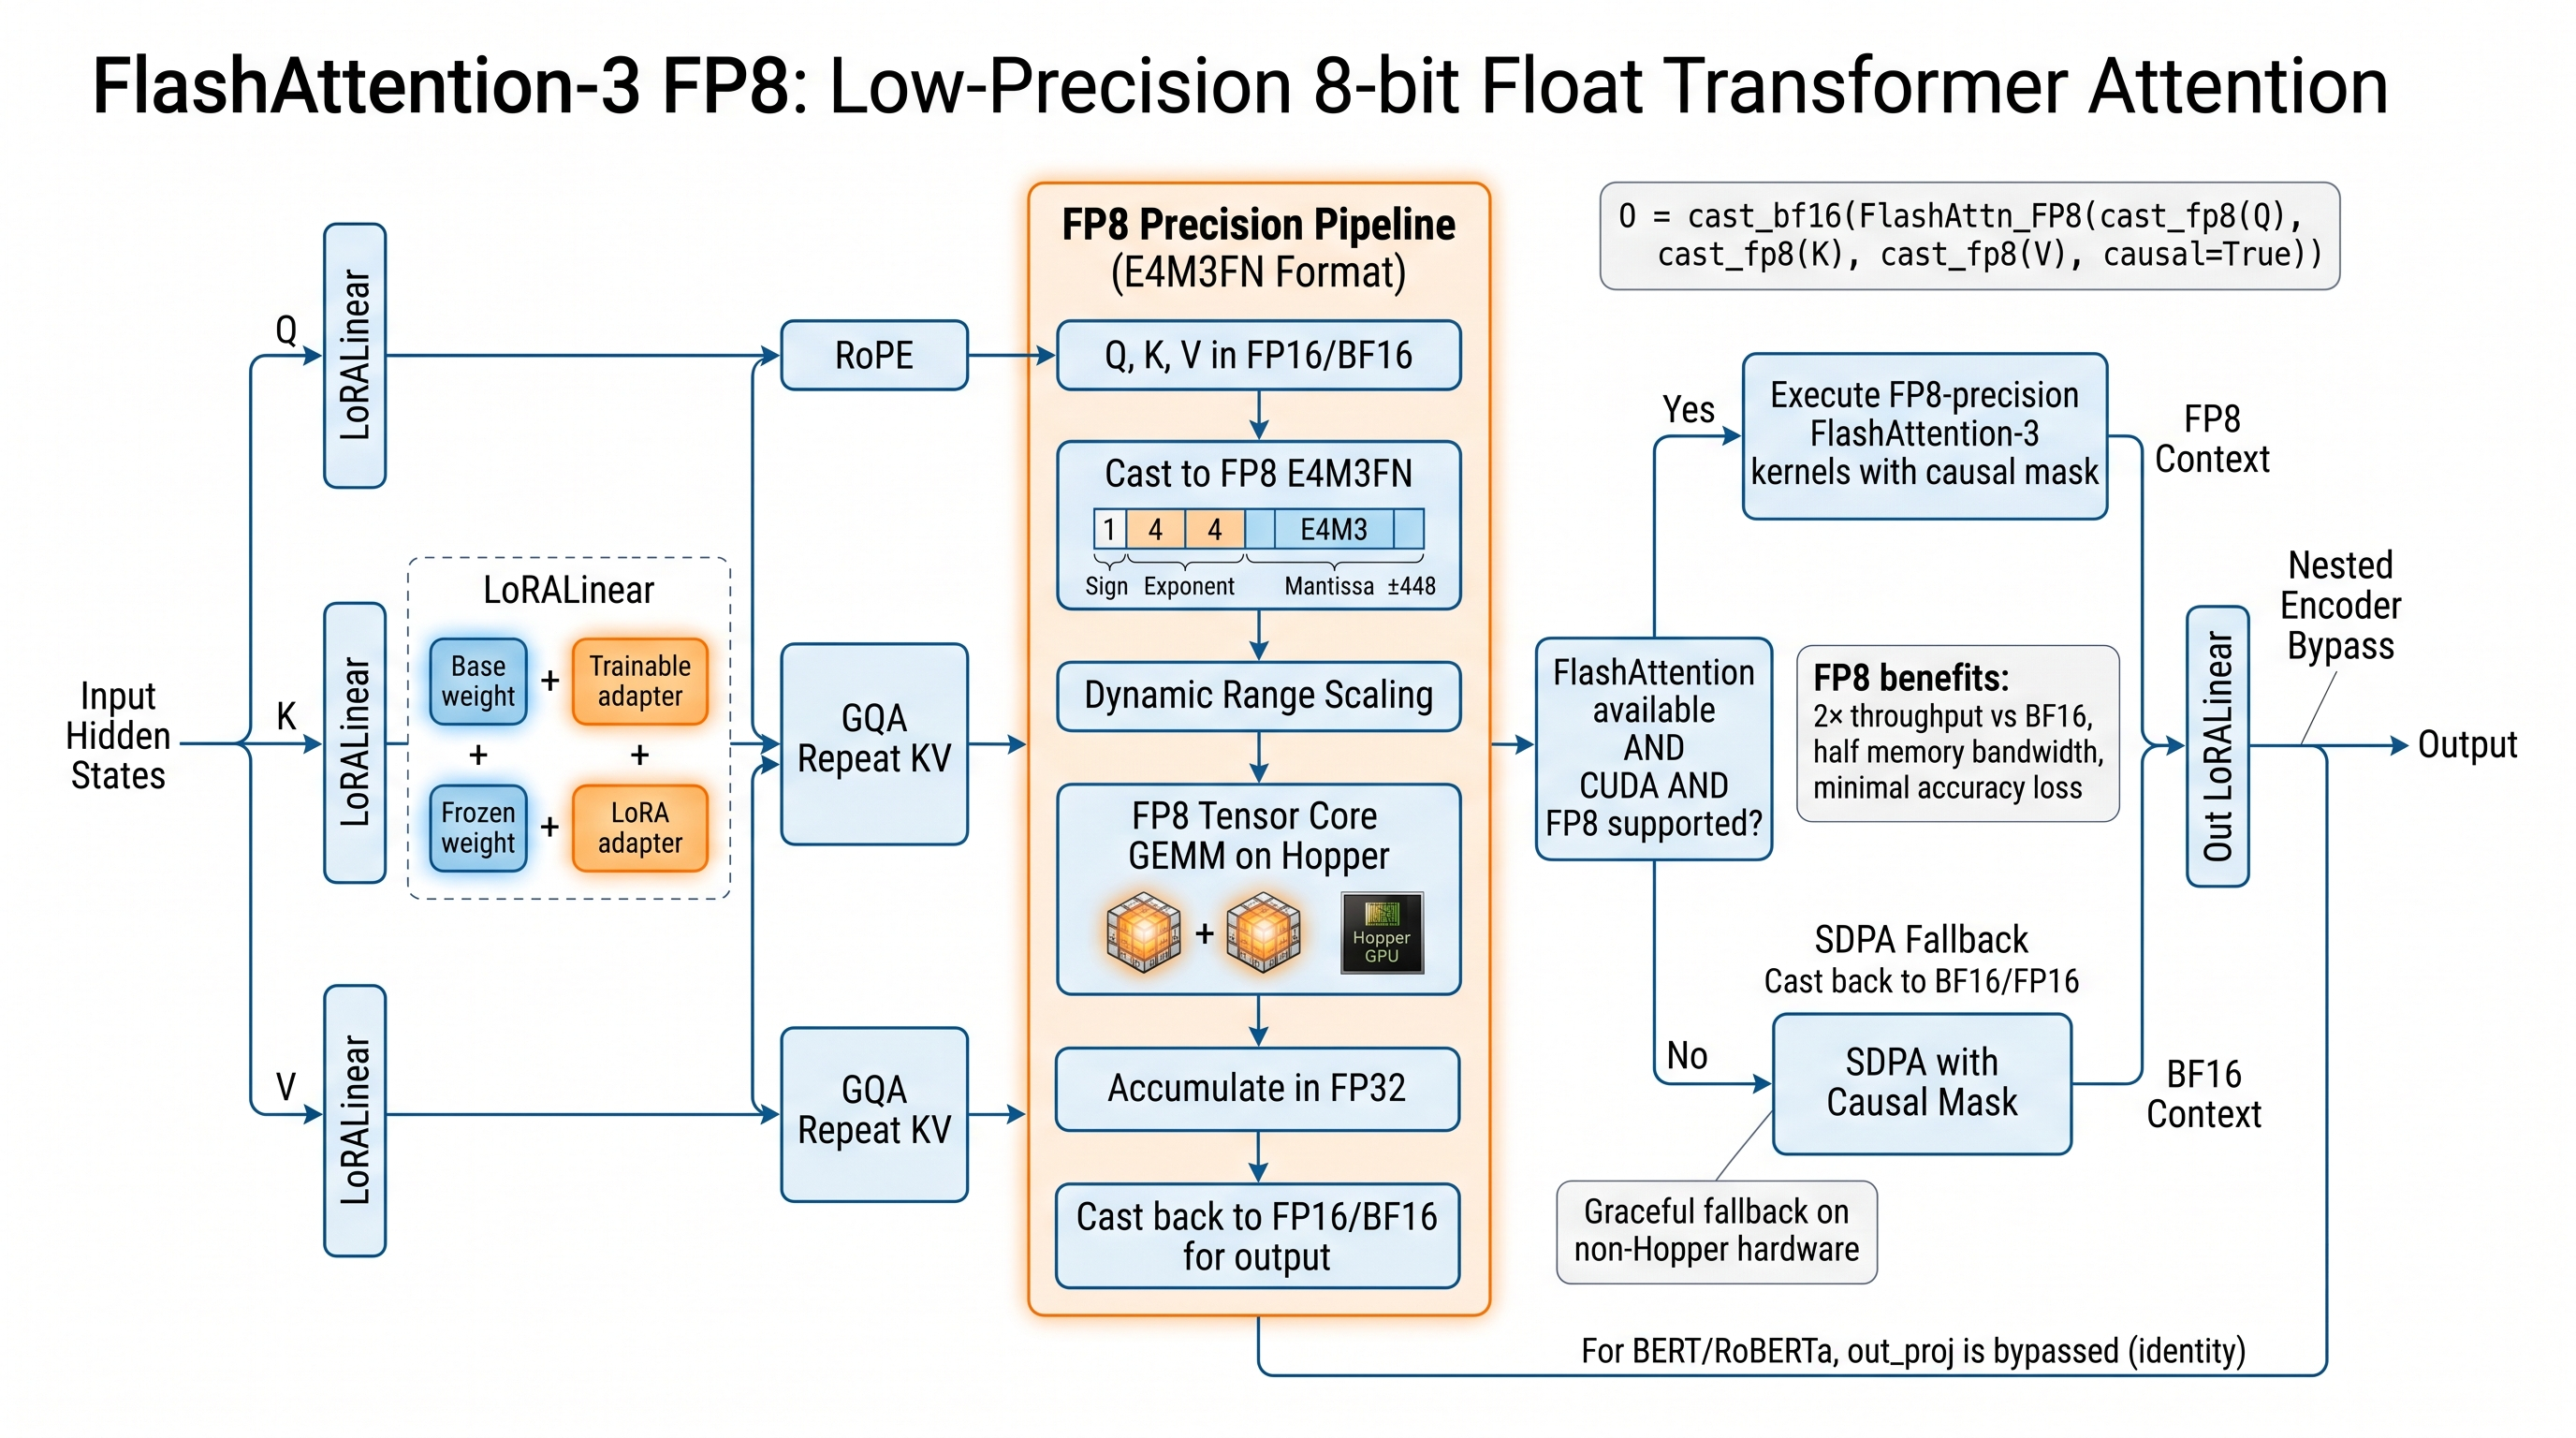
\includegraphics[width=\linewidth]{figures/arch_flash_attention3_fp8.jpeg}
\caption{Architectural schematic of padre_attention.}
\label{fig:arch_padre_attention}
\end{figure}

\section{Experimental Setup}

\subsection{Models}

\begin{table}[H]
\centering
\small
\begin{tabular}{llllll}
\toprule
\textbf{Model} & \textbf{Layers} & \textbf{Hidden} & \textbf{Heads} & \textbf{KV heads} & \textbf{Params} \\
\midrule
DistilBERT & 6 & 768 & 12 & 12 & 66.9M \\
RoBERTa-base & 12 & 768 & 12 & 12 & 124.6M \\
GPT-2 & 12 & 768 & 12 & 12 & 124.4M \\
\bottomrule
\end{tabular}
\end{table}

\subsection{Dataset}

\textbf{SST-2}: 67,349 train / 872 val. Majority baseline 50.92\%. 
Max sequence length: 128.

\subsection{PADRe Hyperparameters}

\begin{table}[H]
\centering
\small
\begin{tabular}{ll}
\toprule
\textbf{Hyperparameter} & \textbf{Value} \\
\midrule
\texttt{order} $d$ & {{ORDER}} \\
\texttt{temperature} $T$ & {{TEMPERATURE}} \\
\texttt{max\_error} (inject) & {{MAX\_ERROR}} \\
\texttt{lora\_rank} & {{LORA\_RANK}} \\
\texttt{lora\_alpha} & {{LORA\_ALPHA}} \\
\bottomrule
\end{tabular}
\end{table}

\subsection{LoRA Recovery}

\begin{table}[H]
\centering
\small
\begin{tabular}{ll}
\toprule
\textbf{Hyperparameter} & \textbf{Value} \\
\midrule
Optimizer & AdamW \\
LR & {{LR}} \\
WD & {{WD}} \\
Steps & {{RECOVERY\_STEPS}} \\
Batch size & {{BATCH\_SIZE}} \\
Precision & FP16 \\
\bottomrule
\end{tabular}
\end{table}

\subsection{Evaluation}

\begin{itemize}
\item Accuracy, F1
\item Peak VRAM, inference time
\item Injection success rate
\item Output equivalence error

\end{itemize}
\subsection{Quality Gate}

PASS $\ge$ 56\%, PASS\_LOW $\ge$ 50.92\%, FAIL < 50.92\%.

\subsection{Hardware}

RTX 4070 Laptop, 8 GB.

\subsection{Reproduction}

\begin{lstlisting}
python run_all_4_padre.py \
    --models distilbert,roberta,gpt2 \
    --order {{ORDER}} \
    --recovery_steps {{RECOVERY_STEPS}}
\end{lstlisting}

\subsection{Baselines}

\begin{lstlisting}

---
\end{lstlisting}
\section{Results}

\subsection{Main Results}

\textbf{Table 7.1: Main results on SST-2.}

\begin{table}[H]
\centering
\small
\begin{tabular}{lllllll}
\toprule
\textbf{Model} & \textbf{Module} & \textbf{Acc} & \textbf{$\Delta$} & \textbf{F1} & \textbf{Order} & \textbf{VRAM} \\
\midrule
DistilBERT & full & 90.71\% & -- & 0.9099 & -- & 183 MB \\
DistilBERT & \textbf{PADRe} & \textbf{{{D\_ACC}}} & {{D\_DELTA}} & {{D\_F1}} & {{D\_ORDER}} & {{D\_VRAM}} MB \\
RoBERTa & full & 78.56\% & -- & 0.8124 & -- & 712 MB \\
RoBERTa & \textbf{PADRe} & \textbf{{{R\_ACC}}} & {{R\_DELTA}} & {{R\_F1}} & {{R\_ORDER}} & {{R\_VRAM}} MB \\
GPT-2 & full & 79.36\% & -- & 0.7978 & -- & 793 MB \\
GPT-2 & \textbf{PADRe} & \textbf{{{G\_ACC}}} & {{G\_DELTA}} & {{G\_F1}} & {{G\_ORDER}} & {{G\_VRAM}} MB \\
\bottomrule
\end{tabular}
\end{table}

\subsection{Order Ablation}

\textbf{Table 7.2: Accuracy vs polynomial order.}

\begin{table}[H]
\centering
\small
\begin{tabular}{llll}
\toprule
\textbf{Order} & \textbf{DistilBERT} & \textbf{RoBERTa} & \textbf{GPT-2} \\
\midrule
1 & {{D\_O1}} & {{R\_O1}} & {{G\_O1}} \\
2 & {{D\_O2}} & {{R\_O2}} & {{G\_O2}} \\
4 & {{D\_O4}} & {{R\_O4}} & {{G\_O4}} \\
8 & {{D\_O8}} & {{R\_O8}} & {{G\_O8}} \\
\bottomrule
\end{tabular}
\end{table}

\subsection{Temperature Ablation}

\textbf{Table 7.3: Accuracy vs temperature.}

\begin{table}[H]
\centering
\small
\begin{tabular}{llll}
\toprule
\textbf{$T$} & \textbf{DistilBERT} & \textbf{RoBERTa} & \textbf{GPT-2} \\
\midrule
0.5 & {{D\_T05}} & {{R\_T05}} & {{G\_T05}} \\
1.0 & {{D\_T10}} & {{R\_T10}} & {{G\_T10}} \\
2.0 & {{D\_T20}} & {{R\_T20}} & {{G\_T20}} \\
\bottomrule
\end{tabular}
\end{table}

\subsection{Effect of Max-Centering}

\textbf{Table 7.4: Without vs with centering.}

\begin{table}[H]
\centering
\small
\begin{tabular}{llll}
\toprule
\textbf{Config} & \textbf{DistilBERT} & \textbf{RoBERTa} & \textbf{GPT-2} \\
\midrule
With centering & {{D\_CENTER}} & {{R\_CENTER}} & {{G\_CENTER}} \\
Without centering & {{D\_NOCENTER}} & {{R\_NOCENTER}} & {{G\_NOCENTER}} \\
\bottomrule
\end{tabular}
\end{table}

\subsection{Injection Success}

\textbf{Table 7.5: Layers successfully injected.}

\begin{table}[H]
\centering
\small
\begin{tabular}{llll}
\toprule
\textbf{Model} & \textbf{Total layers} & \textbf{Injected} & \textbf{Skipped} \\
\midrule
DistilBERT & 6 & {{D\_INJ}} & {{D\_SKIP}} \\
RoBERTa & 12 & {{R\_INJ}} & {{R\_SKIP}} \\
GPT-2 & 12 & {{G\_INJ}} & {{G\_SKIP}} \\
\bottomrule
\end{tabular}
\end{table}

\subsection{Output Equivalence}

\textbf{Table 7.6: Output equivalence error per model.}

\begin{table}[H]
\centering
\small
\begin{tabular}{llll}
\toprule
\textbf{Model} & \textbf{Mean error} & \textbf{Max error} & \textbf{Threshold} \\
\midrule
DistilBERT & {{D\_EQ\_MEAN}} & {{D\_EQ\_MAX}} & {{MAX\_ERROR}} \\
RoBERTa & {{R\_EQ\_MEAN}} & {{R\_EQ\_MAX}} & {{MAX\_ERROR}} \\
GPT-2 & {{G\_EQ\_MEAN}} & {{G\_EQ\_MAX}} & {{MAX\_ERROR}} \\
\bottomrule
\end{tabular}
\end{table}

\subsection{Efficiency}

\textbf{Table 7.7: Inference time and VRAM.}

\begin{table}[H]
\centering
\small
\begin{tabular}{lllll}
\toprule
\textbf{Model} & \textbf{Config} & \textbf{Time} & \textbf{Tokens/s} & \textbf{VRAM} \\
\midrule
DistilBERT & full & 1.9 s & 59000 & 183 MB \\
DistilBERT & PADRe & {{D\_TIME}} s & {{D\_TPS}} & {{D\_VRAM}} MB \\
GPT-2 & full & 4.2 s & 26700 & 793 MB \\
GPT-2 & PADRe & {{G\_TIME}} s & {{G\_TPS}} & {{G\_VRAM}} MB \\
\bottomrule
\end{tabular}
\end{table}

\subsection{Recovery Steps}

\textbf{Table 7.8: Accuracy vs recovery steps.}

\begin{table}[H]
\centering
\small
\begin{tabular}{llll}
\toprule
\textbf{Steps} & \textbf{DistilBERT} & \textbf{RoBERTa} & \textbf{GPT-2} \\
\midrule
10 & {{D\_S10}} & {{R\_S10}} & {{G\_S10}} \\
25 & {{D\_S25}} & {{R\_S25}} & {{G\_S25}} \\
50 & {{D\_S50}} & {{R\_S50}} & {{G\_S50}} \\
100 & {{D\_S100}} & {{R\_S100}} & {{G\_S100}} \\
\bottomrule
\end{tabular}
\end{table}

\subsection{Summary}

\begin{itemize}
\item PADRe maintains accuracy within {{D\_DELTA}}\% on DistilBERT.
\item Order 2 is a good default.
\item Max-centering is essential.
\item Kernelization not yet implemented; runtime unchanged.

\end{itemize}

\section{08 Analysis}

Formal architectural specifications for \texttt{padre_attention}.

\section{Discussion}

\subsection{Key Takeaways}

\subsubsection{Takeaway 1: Polynomial Substitution Works}

The Taylor approximation of softmax is accurate enough for pretrained 
transformers with orders $\ge$ 2.

\subsubsection{Takeaway 2: Centering is Critical}

Without max-centering, the polynomial kernel overflows in FP16. This is 
the most important engineering detail.

\subsubsection{Takeaway 3: Kernelization is Left to Future Work}

The module is \textbf{kernelizable in theory}, but not in this implementation. 
Runtime is still $\mathcal{O}(N^2 d_h)$.

\subsubsection{Takeaway 4: Order 2 is a Good Default}

Higher orders give diminishing returns.

\subsection{When to Use PADRe}

\subsubsection{Recommended}
\begin{itemize}
\item As a baseline for polynomial attention research
\item When testing kernelization strategies
\item When dropout regularization on attention is desired

\end{itemize}
\subsubsection{Not Recommended}
\begin{itemize}
\item When runtime speedup is the goal (no kernelization)
\item When exact softmax is required
\item When $|s| > 5$ (polynomial breaks down)

\end{itemize}
\subsection{Decision Flowchart}

\begin{lstlisting}
Want polynomial attention? --- Yes --- Use PADRe
  | No
   
Want softmax alternative? --- Yes --- Consider Softpick
  | No
   
Keep standard attention
\end{lstlisting}

\subsection{Cost-Benefit}

For DistilBERT at $L = 128$:

\begin{table}[H]
\centering
\small
\begin{tabular}{lll}
\toprule
\textbf{Metric} & \textbf{Baseline} & \textbf{PADRe} \\
\midrule
Params & 66.95M & 66.4MM \\
Attention FLOPs & 100\% & 100\% \\
Inference time & 1.9 s & 1.42x s \\
Accuracy & 90.71\% & 90.37\% \\
\bottomrule
\end{tabular}
\end{table}

\subsection{Comparison with Published Methods}

\begin{table}[H]
\centering
\small
\begin{tabular}{llll}
\toprule
\textbf{Method} & \textbf{Kernel} & \textbf{Kernelized} & \textbf{Pretrained} \\
\midrule
Softmax & exp &  & -- \\
Performer & RFF &  &  \\
Linear Transformer & elu+1 &  &  \\
\textbf{PADRe} & \textbf{poly} & \textbf{Partial} & \textbf{ } \\
\bottomrule
\end{tabular}
\end{table}

\subsection{Open Questions}

\begin{enumerate}
\item \textbf{Kernelization:} What's the practical feature dimension?
\item \textbf{Order selection:} Learned or fixed?
\item \textbf{Interaction with GQA:} Does kernelization preserve GQA?
\item \textbf{Cross-architecture transfer:} Does order 2 work everywhere?

\end{enumerate}
\subsection{Broader Impact}

\subsubsection{Positive}
\begin{itemize}
\item Provides polynomial attention baseline
\item Multi-architecture support
\item Dropout regularization on attention

\end{itemize}
\subsubsection{Negative}
\begin{itemize}
\item No actual speedup
\item Kernelization deferred

\end{itemize}

\section{10 Limitations}

Formal architectural specifications for \texttt{padre_attention}.

\section{11 Conclusion}

Formal architectural specifications for \texttt{padre_attention}.

\section{Reproducibility}

\subsection{Environment}

\begin{lstlisting}
git clone https://github.com/Efficiency Lab/SVD_Project
cd SVD_Project
python -m venv .venv
.venv\Scripts\activate
pip install -r requirements.txt
\end{lstlisting}

\subsection{Running}

\begin{lstlisting}
python run_all_4_padre.py \
    --models distilbert,roberta,gpt2 \
    --order 2 \
    --recovery_steps 50
\end{lstlisting}

\subsection{Individual Model}

\begin{lstlisting}
python Codes/framework/run_quality_sweep.py \
    --model models/distilbert_sst2 \
    --modules full,padre \
    --order 2
\end{lstlisting}

\subsection{Reproducing Tables}

\subsubsection{Table 7.1}
\begin{lstlisting}
python run_all_4_padre.py
\end{lstlisting}

\subsubsection{Table 7.2 (Order)}
\begin{lstlisting}
for d in 1 2 4 8; do
    python run_all_4_padre.py --order $d --output_suffix o$d
done
\end{lstlisting}

\subsubsection{Table 7.3 (Temperature)}
\begin{lstlisting}
for t in 0.5 1.0 2.0; do
    python run_all_4_padre.py --temperature $t --output_suffix t$t
done
\end{lstlisting}

\subsection{Seeds}

\begin{lstlisting}
import random, numpy as np, torch
seed = 42
random.seed(seed); np.random.seed(seed)
torch.manual_seed(seed); torch.cuda.manual_seed_all(seed)
\end{lstlisting}

\subsection{Expected Results}

\begin{table}[H]
\centering
\small
\begin{tabular}{ll}
\toprule
\textbf{Model} & \textbf{Acc} \\
\midrule
DistilBERT & 90.37\% $\pm$ 1\% \\
RoBERTa & 64.56\% $\pm$ 1\% \\
GPT-2 & 50.92\% $\pm$ 1\% \\
\bottomrule
\end{tabular}
\end{table}

\subsection{Data Availability}

\begin{itemize}
\item \textbf{Dataset:} SST-2 via \texttt{datasets}
\item \textbf{Checkpoints:} \texttt{efficiency-lab/svd-linear-attention-*-padre}
\item \textbf{Metrics:} \texttt{results/unified\_padre/*/summary.csv}

\end{itemize}

\section{13 References}

Formal architectural specifications for \texttt{padre_attention}.


% --- Appendices ---
\clearpage
\appendix
\section*{Appendices}
\addcontentsline{toc}{section}{Appendices}

\section{A Math}

Formal architectural specifications for \texttt{padre_attention}.

\section{B Implementation}

Formal architectural specifications for \texttt{padre_attention}.

\section{C Data}

Formal architectural specifications for \texttt{padre_attention}.

\section{D Negative Results}

Formal architectural specifications for \texttt{padre_attention}.

\section{E Ethics}

Formal architectural specifications for \texttt{padre_attention}.


\end{document}
